\documentclass[aspectratio=169]{beamer}

\usetheme{metropolis}
\usepackage{appendixnumberbeamer}

\usepackage{booktabs}
\usepackage[scale=2]{ccicons}

\usepackage{pgfplots}

\usepackage{xspace}
\newcommand{\themename}{\textbf{\textsc{metropolis}}\xspace}

\usepackage[utf8]{inputenc}
\usepackage[T1]{fontenc}

\usepackage{listings}
\usepackage{xcolor, colortbl}
\usepackage{multicol}
\usepackage{chronology}

\usepackage[]{algorithm2e}

\definecolor{done}{rgb}{0.36, 0.72, 0.36}
\definecolor{doing}{rgb}{1.0, 0.8, 0.0}
\definecolor{scheduled}{rgb}{0.25, 0.54, 0.79}

\newcommand{\done}{\cellcolor{done}}
\newcommand{\scheduled}{\cellcolor{scheduled}}
\newcommand{\doing}{\cellcolor{doing}}

\bibliographystyle{unsrt}

\lstdefinestyle{sharpc}{language=[Sharp]C, frame=lr, rulecolor=\color{blue!80!black}}


\title{Eliminando Gargalos de Processamento \newline Utilizando Rust}
\date{}
\author{Johnathan Fercher}
%\institute{Braspag}
\titlegraphic{\hfill
\includegraphics[height=2.0cm]{imgs/logo.png}}

\begin{document}
\maketitle

\begin{frame}{Sumário}
  \setbeamertemplate{section in toc}[sections numbered]
  \tableofcontents[hideallsubsections]
\end{frame}

\section{Introdução}
\begin{frame}{Introdução}
	\begin{center}
		
\includegraphics[width=2.5cm]{imgs/rust.png}
	\end{center}

	Uma linguagem de programação de sistemas que roda incrivelmente rápido, previne falhas de segmentação, e garente segurança entre threads.
\end{frame}

\begin{frame}{Motivação}
	\begin{quote}
		\hspace{0.5cm}"O clock dos processadores dobra a cada 18 meses."
		
		\hspace{8.2cm}Lei de Moore, 1965.
	\end{quote}
\end{frame}

\begin{frame}{Motivação}
	\begin{center}
		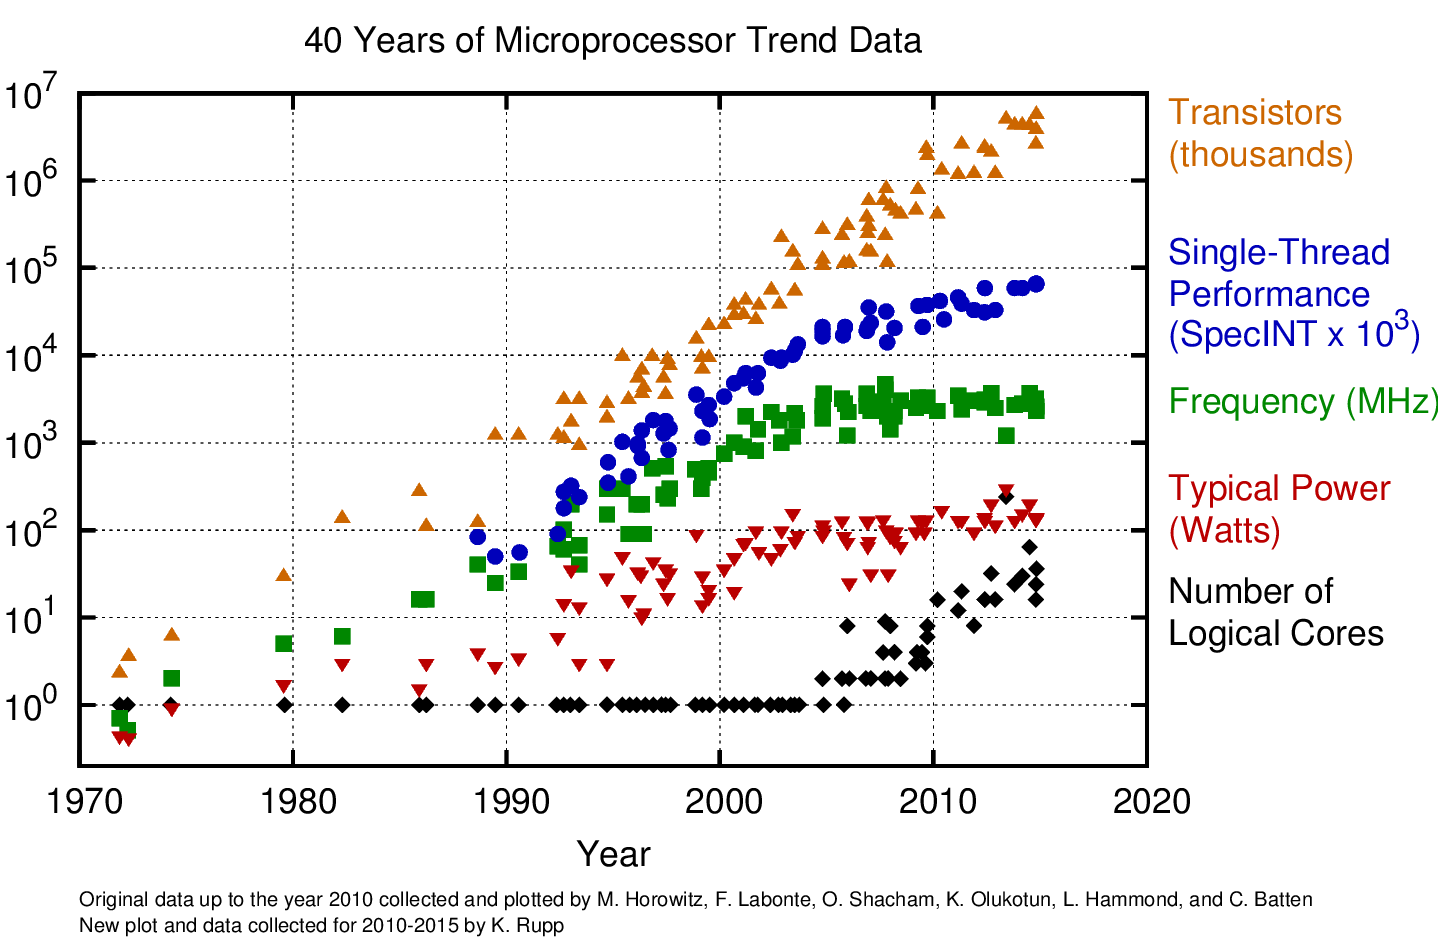
\includegraphics[width=12.5cm]{imgs/cores-history.png}
	\end{center}
\end{frame}

\begin{frame}{Motivação}
	\begin{quote}
		"The way the processor industry is going, is to add more and more cores, but nobody knows how to program those things. I mean, two, yeah; four, not really; eight, forget it."
		
		\hspace{8.2cm}Steve Jobs, Apple.
	\end{quote}
\end{frame}

\begin{frame}{Motivação}
	Programação Paralela
	\begin{center}
		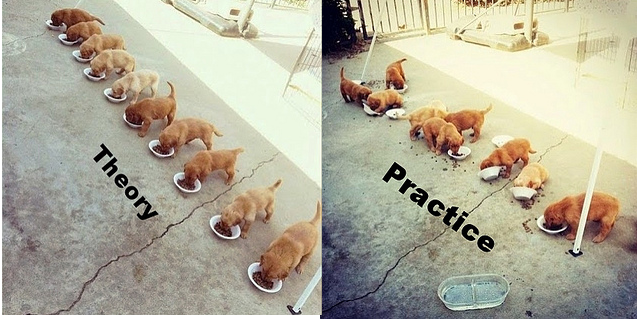
\includegraphics[width=11.5cm]{imgs/meme.png}
	\end{center}
\end{frame}

\begin{frame}{Motivação}
	\begin{center}
		
\includegraphics[width=12.5cm]{imgs/bug.png}
	\end{center}
\end{frame}

\begin{frame}{Motivação}
	Problemas:
	\begin{itemize}
		\item \textcolor{red}{Data races};
		\item Race conditions;
		\item Deadlock;
		\item \textcolor{red}{Use After Free};
		\item \textcolor{red}{Double Free};
	\end{itemize}
\end{frame}

\begin{frame}{História}
	\begin{chronology}[5]{2002}{2015}{80ex}[\textwidth]
		\event[2002]{2003}{C \& LLVM}
		\event{2006}{Graydon Hoare}
		\event{2009}{Mozilla}
		\event{2010}{Rust-c in Rust}
		\event{2011}{Rust-c using LLVM}
		\event{2012}{Alpha}
		\event{2013}{Cargo}
		\event{2015}{Stable}
	\end{chronology}
\end{frame}

\begin{frame}{Desenvolvimento}
	\begin{itemize}
		\item Licença MIT no Github;
		\item Duas versões: Stable e Nightly;
		\item Atualizações a cada 6 semanas;
		\item Processo de RFC;
		\item Quando uma RFC é aprovada ela é adicionada na versão Nightly;
		\item Após algum tempo em Nightly, ela pode ser adicionada na versão Stable, deixada de lado ou alterada;	
	\end{itemize}
\end{frame}

\section{Quem usa? E para que?}

\begin{frame}{Quem usa? E para que?}
	\begin{center}
		
\includegraphics[width=4.5cm]{imgs/dropbox.png}	
		
		"Optimizing cloud file-storage."
	\end{center}
\end{frame}

\begin{frame}{Quem usa? E para que?}
	\begin{center}
		
\includegraphics[width=4.5cm]{imgs/canonical.jpeg}	
		
		"Everything from server monitoring to middleware!"
	\end{center}
\end{frame}

\begin{frame}{Quem usa? E para que?}
	\begin{center}
		
\includegraphics[width=4.5cm]{imgs/smartthings.png}	
		
		"Developing memory-safe embedded applications on our SmartThings Hub and supporting services in the cloud."
	\end{center}
\end{frame}

\begin{frame}{Quem usa? E para que?}
	\begin{center}
		
\includegraphics[width=4.5cm]{imgs/mozilla.png}	
		
		"Building the Servo browser engine, integrating into Firefox, other projects."
	\end{center}
\end{frame}

\begin{frame}{Quem usa? E para que?}
	\begin{center}
		
\includegraphics[width=4.5cm]{imgs/coursera.png}	
		
		"Programming Assignments in secured Docker containers."
	\end{center}
\end{frame}

\begin{frame}{Quem usa? E para que?}
	\begin{center}
		
\includegraphics[width=2.2cm]{imgs/chef.png}	
		
		"Letting you develop, deploy and manage infrastructure, run-time environments and applications."
	\end{center}
\end{frame}

\begin{frame}{Quem usa? E para que?}
	\begin{center}
		
\includegraphics[width=4.5cm]{imgs/atlassian.png}	
		
		"We use Rust in a service for analyzing petabytes of source code."
	\end{center}
\end{frame}

\begin{frame}{Quem usa? E para que?}
	\begin{center}
		
\includegraphics[width=3.0cm]{imgs/npm.jpeg}	
		
		"Replacing C and rewriting performance-critical bottlenecks in the registry service architecture."
	\end{center}
\end{frame}

\begin{frame}{Quem usa? E para que?}
	\begin{center}
		
\includegraphics[width=3.5cm]{imgs/habitat.png}	
		
		"Habitat is automation that travels with the app. Rust aid us to remove bottlenecks."
	\end{center}
\end{frame}

\begin{frame}{Quem usa? E para que?}
	\begin{itemize}
		\item No site oficial da linguagem há mais 123 empresas que deixaram claro que utilizam Rust;
	\end{itemize}
\end{frame}

\section{Sugestões de Regras do Velocity}

\begin{frame}{Velocity}
	Regras de repetição:
	\begin{itemize}
		\item 5 repetições de um \textbf{Cpf} em 10 minutos;
		\item 10 repetições de um \textbf{Cartão} em 2 dias;
		\item 2 repetições de um \textbf{Ip} em 5 minutos;
	\end{itemize}

	\begin{chronology}[5]{1}{10}{80ex}[\textwidth]
		\event{1}{\textbf{1 min:} 127.0.0.1}
		\event{4}{\textbf{4 min:} 127.0.0.1}
		\event{7}{\textbf{7 min:} 127.0.0.1}
		\event{8}{\textcolor{red}{\textbf{8 min:} 127.0.0.1}}
	\end{chronology}
\end{frame}

\begin{frame}{Algoritmo}
	\begin{algorithm}[H]
		var transactions = List<Transaction>()\;
		var quarantine = new DateTime()\;
		\vspace{0.2cm}
		\For{transaction \textbf{in} transactions}{
			\eIf{quarantine\_is\_active(quarantine, transaction)}{
				block(transaction)\;
				update(quarantine)\;
			}{
				\If{extrapolate\_rule(transaction)}{
					block(transaction)\;
					update(quarantine)\;
				}	
			}
		}
	\end{algorithm}
\end{frame}

\begin{frame}{Benchmark (v1.0)}
	\begin{figure}
		\begin{tikzpicture}
		\begin{axis}[
		mbarplot,
		ymin=0, ymax=200.0,
		%xlabel={Foo},
		ylabel={\scriptsize Tempo de Execução},
		width=0.9\textwidth,
		height=8cm,
		xticklabels={,,}
		]
		
		%\addplot plot coordinates {(0, 30.0)};
		\addplot plot coordinates {(0, 300.0)};
		\addplot plot coordinates {(0, 10.0)};
		
		\legend{C\# (300m), Rust (10m)}
		
		\end{axis}
		\end{tikzpicture}
	\end{figure}
\end{frame}

\begin{frame}{Benchmark (v2.0)}
	\begin{figure}
		\begin{tikzpicture}
		\begin{axis}[
		mbarplot,
		ymin=0, ymax=200.0,
		%xlabel={Foo},
		ylabel={\scriptsize Tempo de Execução},
		width=0.9\textwidth,
		height=8cm,
		xticklabels={,,}
		]
		
		%\addplot plot coordinates {(0, 30.0)};
		\addplot plot coordinates {(0, 200.0)};
		\addplot plot coordinates {(0, 76.0)};
		
		\legend{Python (200s), Rust (76s)}
		
		\end{axis}
		\end{tikzpicture}
	\end{figure}
\end{frame}

\section{Hands-On}

\section{Material Complementar}

\begin{frame}{Rust by Example}
	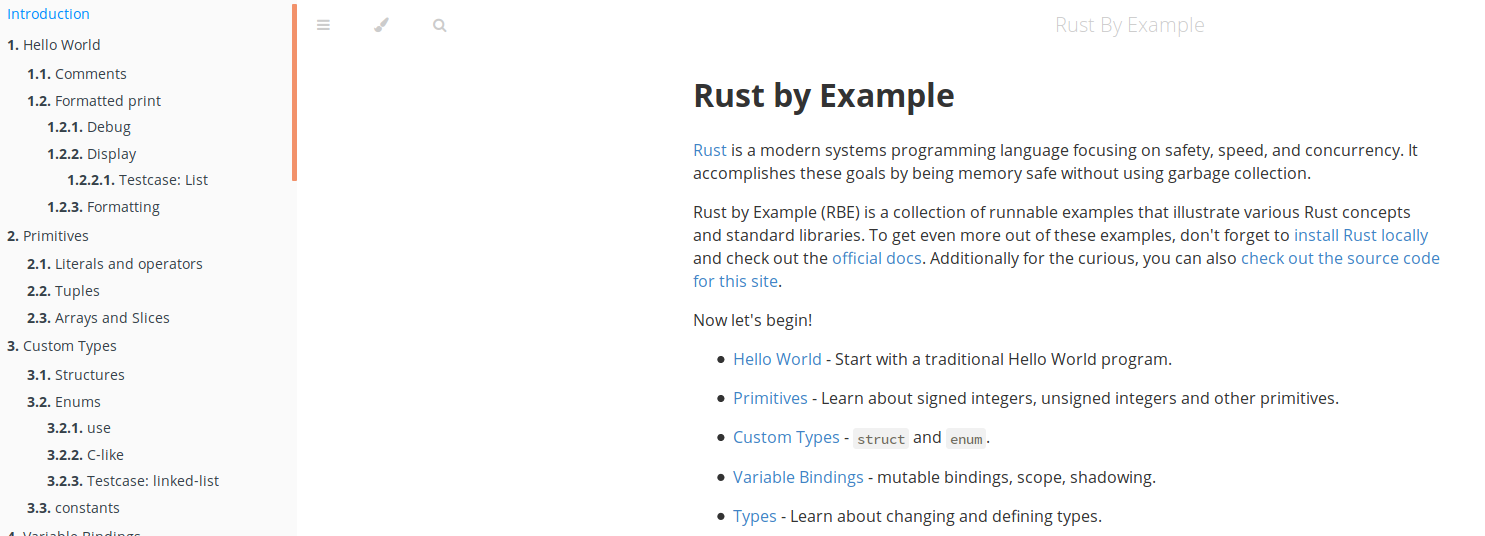
\includegraphics[width=15.0cm]{imgs/rust-by-example.png}	
\end{frame}

\begin{frame}{Rust - Concorrência e alta performance com segurança}
	\begin{center}
		
\includegraphics[width=5.0cm]{imgs/casa-do-codigo-rust.jpg}	
	\end{center}
\end{frame}

\begin{frame}{Programming Rust}
	\begin{center}
		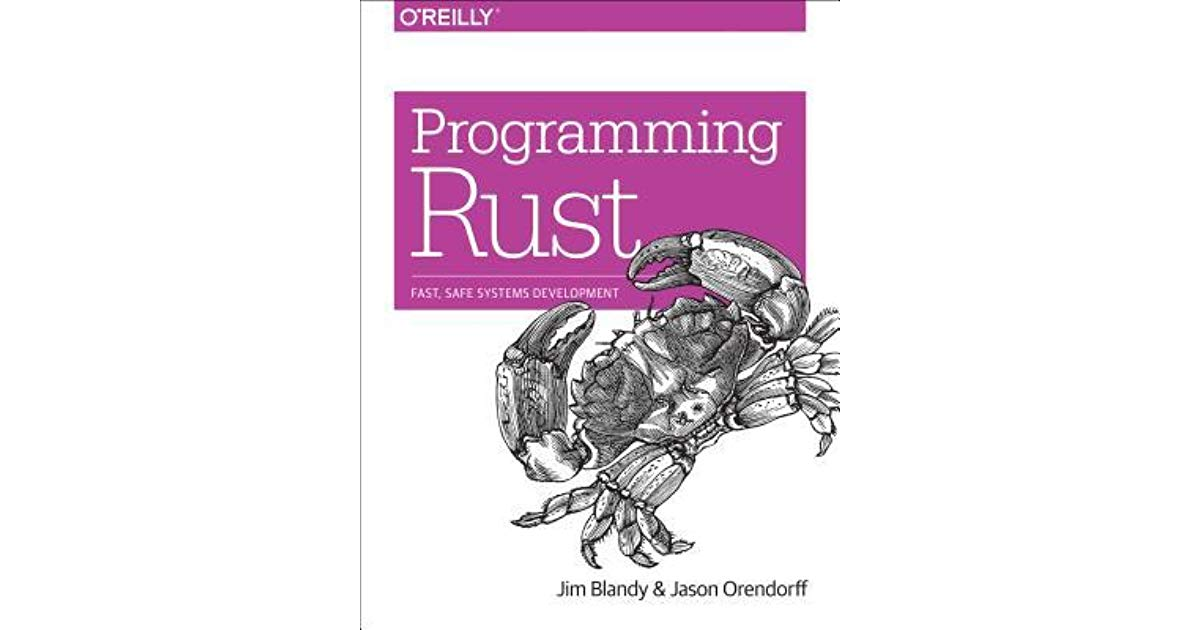
\includegraphics[width=13.0cm]{imgs/programming-rust.jpg}	
	\end{center}
\end{frame}

\begin{frame}{Programming Rust}
	\begin{center}
		
\includegraphics[width=5.0cm]{imgs/hands-on-functional-programming-in-rust.jpg}	
	\end{center}
\end{frame}

\begin{frame}{Eventos}
	\begin{center}
		
\includegraphics[width=4.0cm]{imgs/rustfest.png}
		\hspace{1cm}	
		
\includegraphics[width=5.0cm]{imgs/rustconf.png}	
	\end{center}
\end{frame}

\begin{frame}{Sistema Operacional}
	\begin{center}
		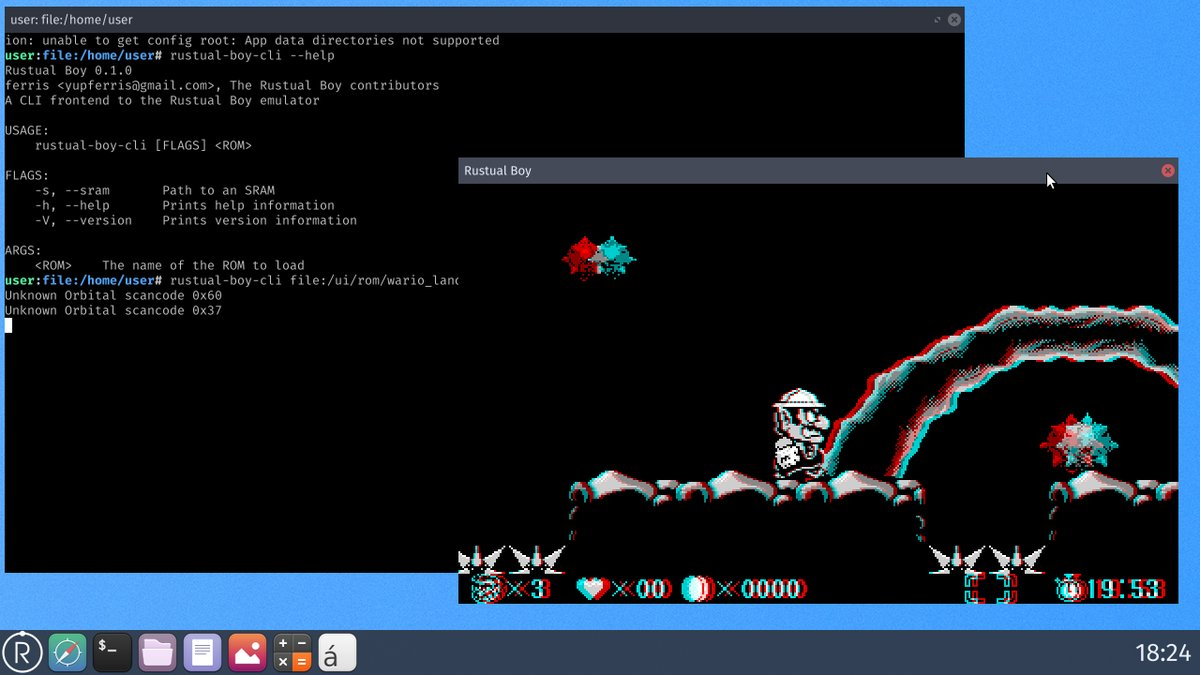
\includegraphics[width=13.0cm]{imgs/redox.jpg}	
	\end{center}
\end{frame}

\begin{frame}[standout]
	\begin{center}
		
\includegraphics[width=2.5cm]{imgs/rustacean.png}
	\end{center}
  	Obrigado
  		
\end{frame}

\end{document}
